\documentclass[11pt]{article}
\usepackage{amssymb,amsmath,lmodern,slashed,cancel}
\usepackage{array}
\usepackage{bm}
\usepackage{graphicx}
\usepackage[hidelinks]{hyperref}
\usepackage[toc,page]{appendix}
\usepackage{footnote,url}
\usepackage{calc}
\usepackage{caption}
\usepackage{xspace}
\usepackage[export]{adjustbox}
\usepackage{subcaption}
\usepackage[margin=.5in,top=1in]{geometry}
\usepackage{fancyhdr}
\pagestyle{fancy}
\lhead{Sid Narayanan}
\rhead{MIT NUPAX Part III}
\chead{\today}
\renewcommand{\headrulewidth}{0.4pt}
\renewcommand{\footrulewidth}{0.4pt}
\newlength\dlf
\newcommand\alignboxed[2]{
  &
  \begingroup
  \settowidth\dlf{$\displaystyle #1$}
  \addtolength\dlf{\fboxsep+\fboxrule}
  \hspace{-\dlf}
  \boxed{#1 #2}
  \endgroup
}
\newcommand\numberthis{\addtocounter{equation}{1}\tag{\theequation}}
\newcommand{\ve}{\mathbf{v}}
\newcommand{\Se}{\mathbf{S}}
\newcommand{\kk}{\vec{k}}
\newcommand{\ue}{\bm{u}}
\newcommand{\sgn}{\text{sgn}}
\newcommand{\p}{\mathbf{p}}
\newcommand{\pop}{\hat{p}}
\newcommand{\x}{\vec{x}}
\newcommand{\vr}{\mathbf{r}}
\newcommand{\xop}{\hat{x}}
\newcommand{\w}{\mathbf{w}}
\newcommand{\z}{\mathbf{z}}
\newcommand{\y}{\vec{y}}
\newcommand{\vq}{\mathbf{q}}
\newcommand{\tv}{\tilde{\ve}}
\newcommand{\vL}{\vec{L}}
\newcommand{\vS}{\vec{S}}
\newcommand{\vso}{\vec{S}^{(1)}}
\newcommand{\vst}{\vec{S}^{(2)}}
\newcommand{\so}{S^{(1)}}
\newcommand{\st}{S^{(2)}}
\newcommand{\vJ}{\vec{J}}
\newcommand{\vl}{\vL}
\newcommand{\vj}{\vJ}
\newcommand{\vjo}{\vec{J}^{(1)}}
\newcommand{\vjt}{\vec{J}^{(2)}}
\newcommand{\jo}{J^{(1)}}
\newcommand{\jt}{J^{(2)}}
\newcommand{\vs}{\vS}
\newcommand{\proj}{\text{\proj}}
\newcommand{\psibar}{\bar{\psi}}
\newcommand{\Psibar}{\bar{\Psi}}
\newcommand{\ubar}{\bar{u}}
\newcommand{\sbar}{\bar{s}}
\newcommand{\nubar}{{\bar{\nu}}}
\newcommand{\vbar}{\bar{v}}
\newcommand{\qbar}{{\bar{q}}}
\newcommand{\fbar}{\bar{f}}
\newcommand{\dbar}{\bar{d}}
\newcommand{\bbar}{\bar{b}}
\newcommand{\cbar}{\bar{c}}
\newcommand{\ebar}{\bar{e}}
\newcommand{\tr}{\text{Tr}}
\newcommand{\spane}{\text{span}}
\newcommand{\ra}{\rangle}
\newcommand{\la}{\langle}
\newcommand{\plus}{|+\ra}
\newcommand{\sulp}{\la+|}
\newcommand{\minu}{|-\ra}
\newcommand{\unim}{\la-|}
\newcommand{\pp}[2]{\dfrac{\partial #1}{\partial #2}}
\newcommand{\ppt}[2]{\dfrac{\partial^2 #1}{\partial #2^2}}
\newcommand{\dd}[2]{\dfrac{d #1}{d #2}}
\newcommand{\fdd}[2]{\dfrac{\delta #1}{\delta #2}}
\newcommand{\fddt}[2]{\dfrac{\delta^2 #1}{(\delta #2)^2}}
\newcommand{\ddt}[2]{\dfrac{d^2 #1}{d #2^2}}
\newcommand{\dre}{\dot{\re}}
\newcommand{\vmu}{\vec{\mu}}
\newcommand{\inv}{^{-1}}
\newcommand{\Mme}{\mathcal{M}}
\newcommand{\La}{\mathcal{L}}
\newcommand{\Jc}{\mathcal{J}}
\newcommand{\E}{\vec{E}}
\newcommand{\B}{\vec{B}}
\newcommand{\Dp}{\frac{d^3p}{(2\pi)^3}}
\newcommand{\Dk}{\frac{d^3k}{(2\pi)^3}}
\newcommand{\Lv}{\mathbf{L}}
\newcommand{\Kv}{\mathbf{K}}
\newcommand{\Lambdahalf}{\Lambda_{\frac{1}{2}}}
\newcommand{\laout}{_\text{out}\la}
\newcommand{\rain}{\ra_\text{in}}
\newcommand{\bv}{\mathbf{b}}
\newcommand{\ddk}{\dfrac{d^d k}{(2\pi)^d}}
\newcommand{\dk}[1]{\dfrac{d^{#1} k}{(2\pi)^{#1}}}
\newcommand{\ddl}{\dfrac{d^d l}{(2\pi)^d}}
\newcommand{\dl}[1]{\dfrac{d^{#1} l}{(2\pi)^{#1}}}
\newcommand{\kslash}{\slashed k}
\newcommand{\nslash}{\slashed n}
\newcommand{\pslash}{\slashed p}
\newcommand{\qslash}{\slashed q}
\newcommand{\lslash}{\slashed l}
\newcommand{\vslash}{\slashed v}
\newcommand{\Dslash}{\slashed D}
\newcommand{\Aslash}{\slashed A}
\newcommand{\eslash}{\slashed \epsilon}
\newcommand{\cf}[2]{c_{#1}^{(#2)}}
\newcommand{\gs}{\text{g.s.}}
\newcommand{\g}[1]{\gamma^{#1}}
\newcommand{\vac}{\text{vac}}
\newcommand{\thetabar}{\bar{\theta}}
\newcommand{\etabar}{\bar{\eta}}
\newcommand{\hov}{\bar{h}}
\newcommand{\Pv}{P_\vslash}
\newcommand{\phicl}{\phi_\text{cl}}
\newcommand{\Veff}{V_\text{eff}}
\newcommand{\C}{\mathbb{C}}
\DeclareMathOperator{\Tr}{Tr}
\DeclareMathOperator{\Trd}{tr} %dirac trace
\DeclareMathOperator{\Li}{Li}
\DeclareMathOperator{\U}{U}
\DeclareMathOperator{\SU}{SU}
\DeclareMathOperator{\su}{\mathfrak{su}}
\DeclareMathOperator{\hc}{h.c.}
\DeclareMathOperator{\erf}{erf}
\DeclareMathOperator{\csch}{csch}
\DeclareMathOperator{\SO}{SO}
\newcommand{\LIPS}{\mathrm{LIPS}}
\newcommand{\F}{\mathcal{F}}
\newcommand{\bigv}{\vphantom{\begin{pmatrix}a\\b\end{pmatrix}^T}}
\newcommand{\fd}[1]{\left[d#1\right]}
\newcommand{\J}{\mathcal{J}}
\newcommand{\Y}{\mathcal{Y}}
\newcommand{\dop}[1]{\Delta_{#1}}
\newcommand{\Z}{\mathbb{Z}}
\newcommand{\Op}{\mathcal{O}}
\newcommand{\chibar}{\bar{\chi}}
\newcommand{\Ham}{\mathcal{H}}
\newcommand{\bipartial}{\barerset\leftrightarrow{\partial}}
\newcommand{\diff}[1]{\dfrac{d^3#1}{(2\pi)^{3/2}(2\omega_{#1})^{1/2}}}
\newcommand{\difft}[2]{\dfrac{d^3#1~d^3#2}{(2\pi)^{3}(2\omega_{#1})^{1/2}(2\omega_{#2})^{1/2}}}
\newcommand{\R}{\mathbb{R}}
\newcommand{\df}[2]{\dfrac{\delta #1}{\delta #2}}
\newcommand{\T}{\mathbf{T}}
\newcommand{\magpi}{|\vec p_i|}
\newcommand{\magpf}{|\vec p_f|}
\newcommand{\gev}{\text{GeV}}
\newcommand{\ev}{\text{eV}}
\newcommand{\nm}{\text{nm}}
\newcommand{\ns}{\text{ns}}
\newcommand{\s}{\text{s}}
\newcommand{\mum}{\mu\text{m}}
\newcommand{\mus}{\mu\text{s}}
\newcommand{\mm}{\text{mm}}
\newcommand{\fm}{\text{fm}}
\newcommand{\cm}{\text{cm}}
\newcommand{\m}{\text{m}}
\newcommand{\km}{\text{km}}
\newcommand{\kev}{\text{keV}}
\newcommand{\mev}{\text{MeV}}
\newcommand{\tev}{\text{TeV}}
\newcommand{\ba}{\text{b}}
\newcommand{\nb}{\text{nb}}
\newcommand{\pb}{\text{pb}}
\newcommand{\gevp}{\text{GeV}/c}
\newcommand{\gevm}{\text{GeV}/c^2}
\newcommand{\msw}{\text{MSW}}
\newcommand{\cnub}{\text{C$\nu$B}}
\newcommand{\sun}{\text{Sun}}
\newcommand{\earth}{\text{Earth}}
\newcommand{\pow}[1]{\times 10^{#1}}
\newcommand{\theend}[1]{
    \begin{center}
    \vspace{#1mm}
    $\mathfrak{THE~END}$
    \end{center}
}
\newcommand{\CP}{\ensuremath{CP}\xspace}
\newcommand{\el}{\ensuremath{e^{-}}\xspace}
\newcommand{\pos}{\ensuremath{e^{+}}\xspace}
\newcommand{\ord}[1]{\ensuremath{\mathcal{O}(#1)}}
\newcommand{\thus}{\ensuremath{~\Rightarrow~}}
\newcommand{\embedimg}[1]{\begin{center}\includegraphics[width=0.48\textwidth]{#1}\end{center}}
\newcommand{\embedimgw}[2]{\begin{center}\includegraphics[width=#2\textwidth]{#1}\end{center}}
\newcommand{\lrad}{\ensuremath{L_\text{rad}}}
\newcommand{\bibspace}{\vspace{5mm}\\\noindent}
\setcounter{section}{-1}
\nonstopmode
\begin{document}

\title{Notes for MIT NUPAX Oral Exam}
\date{Last modified: \today}
\author{Siddharth Narayanan, MIT}

\maketitle

\tableofcontents

\section{General information}
\subsection{Chirality}
\begin{itemize}
  \item The chirality operators are
  \begin{equation}
    P_R = \frac{1}{2} \left(1+\gamma^5\right), \quad P_L = \frac{1}{2} \left(1-\gamma^5\right)
  \end{equation}
  \item Note $P_R+P_L = I$
  \item $P_{R,L}$ projects $u$ onto $u_{R,L}$ and $v$ onto $v_{L,R}$ (note the action is reversed for antiparticles)
  \item In the massless (relativistic) limit, chirality becomes helicity ($\vec\sigma \cdot \vec p / |\vec p|$)
\end{itemize}

\section{Discrete symmetries}
\subsection{Parity}

\begin{itemize}
  \item The parity operator flips space dimensions:
  \begin{equation}
    P \psi(\x,t)\mapsto \psi(-\x,t)
  \end{equation}
  \item Clearly $P$ is hermitian and unitary
  \item For Dirac spinors, $P = \gamma^0 = \begin{pmatrix} I & \\ & -I \end{pmatrix}$
  \item Parity is conserved in QED:
  \begin{itemize}
    \item Matrix element for $\el q \rightarrow \el q$ scattering is:
    \begin{equation}
      \Mme = \frac{Q_qe^2}{q^2}j_e \cdot j_q, \quad j_x^\mu = \ubar(p_{x,f})\gamma^\mu u(p_{x,i})
    \end{equation}
    \item Applying $P$ to the spinors:
    \begin{equation}
      u \rightarrow \gamma^0 u, \quad \ubar = u^\dag\gamma^0 \rightarrow u^\dag {\gamma^0}^\dag \gamma^0 = \ubar \gamma^0
    \end{equation}
    \item So the currents transform as ($k$ is a spatial coordinate):
    \begin{equation}
      j_x^0 \rightarrow j_x^0, \quad j_x^k \rightarrow -j_x^k
    \end{equation}
    \item The minus sign in the spatial component cancels when taking the inner product, so $P:\Mme \mapsto \Mme$
  \end{itemize}
  \item Consider the decay of $\rho^0(1^-)$ to a pair of charged pions $(0^-)$. 
  \begin{itemize}
    \item Because the decay starts in the $J=1$ state, the orbital angular momentum of the pion system must be $1$. ($P = (-1)^l = -1$)
    \item This decay is allowed, since parity is conserved: $P(\rho^0) = P(\pi^+)P(\pi^-)(-1)^l = -1$
  \end{itemize}
  \item Now consider the decay of $\eta(0^-)$ to a pair of charged pions
  \begin{itemize}
    \item The final orbital angular momentum is $l=0$
    \item This decay is forbidden, since parity is violated: $P(\eta) \neq P(\pi^+)P(\pi^-)(-1)^l = 1$
  \end{itemize}
  \item \thus parity is not conserved in the weak interaction
\end{itemize}

\subsection{$CPT$}
\begin{itemize}
  \item In general, Lorentz-invariant QFTs must be invariant under $CPT$
  \begin{itemize}
    \item This is why particles have identical masses and magnetic moments
  \end{itemize}
\end{itemize}

\section{Flavor symmetry and the quark model}

\subsection{Isospin and flavor symmetry}
\begin{itemize}
  \item The nuclear force (i.e. residual strong force) is approximately charge-independent:
  \begin{equation}
    V_{pp} \sim V_{np} \sim V_{nn}
  \end{equation}
  \begin{itemize}
    \item The masses of the neutron and proton are very close
    \item Motivates an approximate symmetry for the strong interaction, known as (nuclear) isospin rotations. Define the proton as the isospin-up state and the neutron as the isospin-down state
  \end{itemize}
  \item The same idea can be extended to quarks
  \begin{itemize}
    \item If we assume that the EM strength for quarks in baryons is much weaker than the strong interaction, then we can impose an (approximate) symmetry for rotations in $q = \begin{pmatrix} u \\ d \end{pmatrix}$ space
    \item Symmetry is approximate even if we drop the EM interaction since $m_u\neq m_d$
    \item This is the isospin $\T = \frac{1}{2}\bm\sigma$. The Hamiltonian is invariant under rotations by $\exp[i\bm\alpha\cdot\T]$, for a real vector $\bm\alpha$. 
    \item $T_i$ therefore generate the $\su(2)$ Lie algebra
  \end{itemize}
  \item We know bound states must consist of 2 or 3 quarks
  \begin{itemize}
    \item Adding two isospin-half states gives an isospin triplet $(T=1)$ and an isospin singlet ($T=0$)
    \item Adding three isospin-half states gives an isospin quadruplet ($T=3/2$) and \emph{two} isospin doublets ($T=1/2$). Note that the doublets are not states of definite symmetry
    \begin{itemize}
      \item However, one of the isospin doublets is symmetric under $1\leftrightarrow2$ (the $1,2$ system has isospin $1$), so call it $\phi_S\left(\frac{1}{2},T_3\right)$
      \item The other isospin doublet is antisymmetric under $1\leftrightarrow2$ (the $1,2$ system has isospin $0$), so call it $\phi_A\left(\frac{1}{2},T_3\right)$
    \end{itemize}
    \item Spin states also decompose in the same way (since spin is also $\SU(2)$)
  \end{itemize}
  \item Antiquark isospin
  \begin{itemize}
    \item Want to define an antiquark vector $\qbar$ such that it transforms in the same way as $q$. That is:
    \begin{equation}
      q \rightarrow U q \thus \qbar \rightarrow U \qbar
    \end{equation}
    \item This is done by defining $\qbar = \begin{pmatrix} - \dbar \\ \ubar \end{pmatrix}$.
    \item The ability to put $q,\qbar$ in the same representation is special to $\SU(2)$
  \end{itemize}
\end{itemize}

\subsection{Building baryons and mesons}
\subsubsection{Baryons ($ud$) in the ground state}
\begin{itemize}
  \item The total wavefunction looks like:
  \begin{equation}
    \psi = \text{flavor}\times\text{spin}\times\text{color}\times\text{space}
  \end{equation}
  \item It can be shown that the color wavefunction is always antisymmetric. If we only consider the $L=0$ ground state, then the space wavefunction is symmetric ($(-1)^l$). Therefore, flavor$~\times~$spin must be symmetric, since the quarks are identical fermions (assuming the flavor symmetry)
  \item Ways of building symmetric $\phi_\text{flavor}\chi_\text{spin}$:
  \begin{itemize}
    \item Symmetric $\phi$ ($T=3/2$) and symmetric $\chi$ ($S=3/2$). This gives four distinct baryons (note $\ni$ is used to describe the quark content without writing down the full wavefunction):
    \begin{equation}
      \Delta^- = ddd,\quad
      \Delta^0 \ni udd,\quad
      \Delta^+ \ni uud,\quad
      \Delta^{++} = uuu
    \end{equation}
    \item Using the symmetrized wavefunctions 
    \begin{equation}
    \dfrac{1}{\sqrt2}\left[\phi_S\left(\frac{1}{2},T_3\right)\chi_S\left(\frac{1}{2},S_3\right)+\phi_A\left(\frac{1}{2},T_3\right)\chi_A\left(\frac{1}{2},S_3\right)\right]
    \end{equation}
    The choice of $T_3$ gives two baryons:
    \begin{equation}
      p \ni uud, \quad n \ni udd
    \end{equation}
  \end{itemize}
\end{itemize}

\subsubsection{Mesons}
\begin{itemize}
  \item Bound state of a quark and antiquark \thus four possible isospin states
  \item The $T=1$ states are the pions:
  \begin{equation}
    \pi^- = d\ubar,\quad \pi^0 = \frac{1}{\sqrt2} (u\ubar-d\dbar),\quad \pi^+ = u\dbar
  \end{equation}
\end{itemize}

\subsection{$\SU(3)$ flavor symmetry}
\begin{itemize}
  \item $ud$ symmetry can be extended to include strange quark
  \begin{itemize}
    \item $m_s - m_{u/d}\sim100~\mev$, which is not insignificant, but is small relative to binding energies of baryons $\sim\gev$
    \item Strong hamiltonian is still invariant under $uds$, but the kinetic terms are less invariant than they were under the $ud$ symmetry
    \item Needs to be treated as an \emph{approximate} symmetry
  \end{itemize}
  \item Define the generators as $T_i = \frac{1}{2}\lambda_i$, where $\lambda_i$ are the Gell-Mann matrices
  \begin{itemize}
    \item $\lambda_{1,2,3}$ are the Pauli $\sigma_{1,2,3}$ matrices for the first two dimensions (i.e. $u,d$) \thus $T_3$ is still the third component of isospin. $T_3s = 0$
    \item $\lambda_{4,5,6,7}$ are (some of) the Pauli matrices for rotations between the other dimensions (i.e $u,s$ and $d,s$)
    \item Turns out that the $9$ generators of the three $\SU(2)$ subgroups of $\SU(3)$ are not all independent. We allow $u,d$ to retain all three of its generators and define $\lambda_8$ as a linear combination of the third generator for the other two subgroups
  \end{itemize}
  \item Since $[T_3,T_8]=0$, we define two (simultaneous) quantum numbers:
  \begin{equation}
    T_3 = \frac{1}{2}\lambda_3,\quad Y = \frac{1}{\sqrt3}\lambda_8
  \end{equation}
  where $Y$ is the flavor hypercharge
  \item The remaining generators can be used to define ladder operators that step between $u\leftrightarrow d$, $d\leftrightarrow s$, $u\leftrightarrow s$
  \item The values of $T_3,Y$ for the quarks and antiquarks make a triangle:
  \embedimgw{figs/su3_t3y.png}{.6}
\end{itemize}

\subsection{Light $uds$ mesons}
\begin{itemize}
  \item This diagram shows a cute way of writing down all $q\qbar$ combinations and getting their $T_3,Y$:
  \embedimgw{figs/mesons1.png}{.6}
  \begin{itemize}
    \item Note that the three states in the middle are not physical (i.e. definite isospin)
    \item To get the physical states (linear combinations of $u\ubar,d\dbar,s\sbar$), we can act the raising/lowering operators on the edge states. This, however, only gives two linearly independent states
    \item Therefore, one of the linear combinations must be in a different rep of $\SU(3)$. It turns out the rep is the $T^2=0$ rep (here $\T$ refers to the vector of $\SU(3)$ generators). The wavefunction is what one would expect:
    \begin{equation}
      \frac{1}{\sqrt3} \left(u\ubar+d\dbar+s\sbar\right)
    \end{equation}
  \end{itemize}
\end{itemize}

\subsubsection{$l=0$}
\begin{itemize}
  \item We now play the game of constructing the meson wavefunction (as was done for baryons). Note there are no Fermi statistics to deal with in this case
  \item We assume $l=0$
  \item There are two possible spin states $s=0,1$. Since $l=0$, we can say $J=0,1$.
  \item The parity of the meson is:
  \begin{equation}
    P(q\qbar') = +1\times -1 \times (-1)^{l=0} = -1
  \end{equation}
  We therefore refer to $J^P = 0^-$ mesons as pseudoscalars and $J^P = 1^-$ as vectors (recall vectors have $P=-1$)
  \item The mesons are shown, split up by pseudoscalars (left) and vectors (right):
  \embedimgw{figs/mesons2.png}{.6}
  \item The $\pi^0$ is as identified in $\SU(2)$: $\frac{1}{\sqrt{2}}(u\ubar-d\dbar)$. The $\eta'$ has a high mass ($\sim1~\gev$) and corresponds to the singlet state identified above. Finally, the $\eta$ is the remaining orthogonal state. Note these three physical states in reality have very different masses (which the $\SU(3)$ theory does not predict) since $m_s \neq m_{u,d}$
  \item The prediction gets worse for the vector $T_3 = Y = 0$ states. We get (experimentally) the physical states:
  \begin{equation}
    \rho^0 = \frac{1}{\sqrt2} (u\ubar - d\dbar), \quad \omega = \frac{1}{\sqrt2}(u\ubar+d\dbar), \quad \phi = s\sbar
  \end{equation}
  Note the $\rho^0$ is kind of an excited state of the $\pi^0$
\end{itemize}

\begin{center}
  \begin{tabular}{l|c}
   $J^P = 0^-$ meson & Mass [MeV]\\ \hline
   $\pi^0$ & 135 \\
   $\pi^\pm$ & 140 \\
   $K^\pm$ & 494 \\
   $K^0,\bar K^0$ & 498 \\
   $\eta$ & 548 \\
   $\eta'$ & 958 \\
  \end{tabular}\quad
  \begin{tabular}{l|c}
   $J^P = 1^-$ meson & Mass [MeV]\\ \hline
   $\rho^0$ & 775 \\
   $\rho^\pm$ & 775 \\
   $K^{*\pm}$ & 892 \\
   $K^{*0},\bar K^{*0}$ & 896 \\
   $\omega$ & 783 \\
   $\phi$ & 1020 \\
  \end{tabular}
\end{center}  

\subsection{Light $uds$ baryons}
\begin{itemize}
  \item Once again, we assume $l=0$
  \item Note that the parity for baryons is $+1 = (+1)^3\times (-1)^{l=0}$
  \item The possible values of $J^P$ therefore are $\frac{1}{2}^+, \frac{3}{2}^+$
  \item We can construct the following irreps by applying the $\SU(3)$ ladder operators to $\SU(2)$ extremal states:
  \begin{itemize}
    \item A decuplet (which contains the deltas). It contains symmetric states. $T = 5/2$
    \item Two octuplets of mixed symmetry. $T = 3/2$
    \item A singlet which is totally antisymmetric. $T = 1/2$. Note: the state contains $uds$, so it cannot be created from a $\SU(2)$ extremal state. 
  \end{itemize}
  \item Physical states must be antisymmetric in the quarks. Recall we need flavor$~\times~$spin to be symmetric. The result is:
  \begin{itemize}
    \item A decuplet from the isospin decuplet
    \item An octuplet formed from linear combinations of states in the two isospin octuplets
    \item This exhausts everything except the isospin singlet state. However, there is no way to form a totally antisymmetric spin state out of three spin-half particles, so it does not correspond to a physical state
  \end{itemize}
\end{itemize}
  \embedimgw{figs/baryons_uds.png}{.6}
  \begin{center}\begin{tabular}{c|lc|lc}
  $s$ quarks & Octet & Mass [GeV] & Decuplet & Mass [GeV]\\\hline
  0 & $p,n$ & 0.94 & $\Delta$ & 1.2\\
  1 & $\Sigma$ & 1.2 & $\Sigma^*$ & 1.4\\
  1 & $\Lambda$ & 1.1 \\
  2 & $\Xi$ & 1.3 & $\Xi^*$ & 1.5 \\
  3 &&& $\Omega$ & 1.7
  \end{tabular}\end{center}

\subsubsection{Baryon magnetic moment}
\begin{itemize}
  \item Define the nuclear magneton:
  \begin{equation}
    \mu_N = \frac{e\hbar}{2m_p}
  \end{equation}
  \item The magnetic moments for a baryon $b$ is calculated by writing out the wavefunction $|b\uparrow\ra$ in terms of the up/down states of the constituent quarks and computing:
  \begin{equation}
    \la b\uparrow | \mu_z | b\uparrow\ra
  \end{equation}
  The quark magnetic moments are computed as:
  \begin{equation}
    \mu_q = \la q\uparrow | \mu_z | q\uparrow\ra = - \la q\downarrow | \mu_z | q\downarrow\ra
  \end{equation}
  \item The moments for protons and neutrons are:
  \begin{equation}
    \mu_p = 2.79\mu_N,\quad \mu_n = -1.9\mu_N
  \end{equation}
\end{itemize}

\section{QCD and $\SU(3)$}
\begin{itemize}
  \item QCD is the QFT of the strong interaction
    \item Mediated by gluons, which are massless gauge bosons corresponding to a local $\SU(3)$ symmetry
    \item Quarks lie in the fundamental rep of $\SU(3)$. The three basis vectors are labeled red, blue, green, and the generators are the usual Gell-Mann matrices:
    \begin{equation}
      T^a = \frac{1}{2}\lambda_a
    \end{equation}
    \item Antiquarks are in the adjoint rep and the basis vectors are $\bar r,\bar g, \bar b$
    \item Because $\SU(3)$ is non-Abelian, there are gluon self-interactions:
    \embedimgw{figs/qcdvertices.png}{.6}
    \item There are 8 physical gluon states, corresponding to the 8 Gell-Mann matrices
    \begin{itemize}
      \item 6 are of the form $c\cbar'$, where $c,c'$ are distinct colors
      \item The other two correspond to $\lambda_3,\lambda_8$ and are $\frac{1}{\sqrt2}(r\bar r-g\bar g)$ and $\frac{1}{\sqrt6}(r\bar r + g\bar g + 2b\bar b)$
    \end{itemize}
\end{itemize}

\subsection{Color confinement}
\begin{itemize}
  \item Particles must always exist in color singlet states 
  \item Has not been proven theoretically, but a qualitative argument can be made:
  \begin{itemize}
    \item Unlike the $\E$-field of two charges being pulled apart, the strong field lines do not spread apart in space, due to gluon self-interaction:
    \embedimgw{figs/qcdfieldlines.png}{.6}
    \item Therefore, the energy grows linearly with the distance (experimentally $\sim 1~\gev/\fm$)
    \item Gluons split into quarks, making color singlet states
  \end{itemize}
  \item Implies gluons cannot travel over macroscopic distances, as they carry color
  \item As with flavor $\SU(3)$ symmetry, can define two quantum numbers $T_3^c,Y^c$ to characterize color $\SU(3)$ symmetry.
  \begin{itemize}
    \item Adding two quarks together gives an octuplet and a singlet:
    \embedimgw{figs/mesoncolor.png}{0.6}
    \item Similarly, adding three quarks (or three antiquarks) gives a decuplet, two octuplets, and a singlet:
    \embedimgw{figs/baryoncolor.png}{0.6}
    \item Only the singlet states correspond to physical states
  \end{itemize}
  \item Hadronization
  \begin{itemize}
    \item If two quarks are produced (say $\gamma\rightarrow q\qbar$) and the quarks have high energy, they will fly apart
    \item However, the interaction of the gluon field between them has a high energy density ($1~\gev/fm$), and so the gluons split into quarks
    \item This process repeats until all of the quarks are bound in, color singlet states
  \end{itemize}
\end{itemize}

\subsection{Running of $\alpha_S$}
\begin{itemize}
  \item Coupling constants run due to higher order corrections made to boson propagators
  \begin{itemize}
    \item The size of these corrections is necessarily dependent on $q^2$
    \item We absorb this $q^2$ dependence into the coupling constant, e.g. $\alpha\rightarrow\alpha(q^2)$, $\alpha_S\rightarrow \alpha_S(q^2)$
  \end{itemize}
  \item At low energies, $\alpha_S \sim \ord1$
  \item Because of the non-Abelian structure of gluon interactions, the $q^2$ evolution of $\alpha_S$ depends on 
  \begin{equation}
    B = \frac{11N_c-2N_f}{12\pi}
  \end{equation}
  In the SM, $B>0$ \thus $\alpha_S$ decreases as a function of $q^2$
  \item This is in contrast with QED, which gets stronger at short distances/high energies:
  \begin{center}
    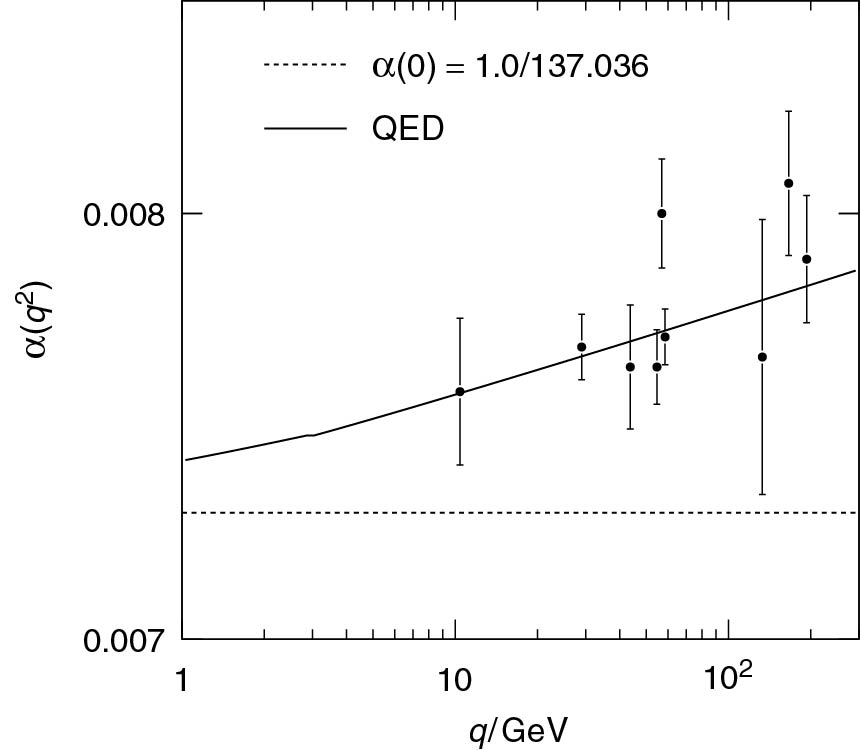
\includegraphics[width=0.32\textwidth]{figs/alpharun.png}\hspace{5mm}
    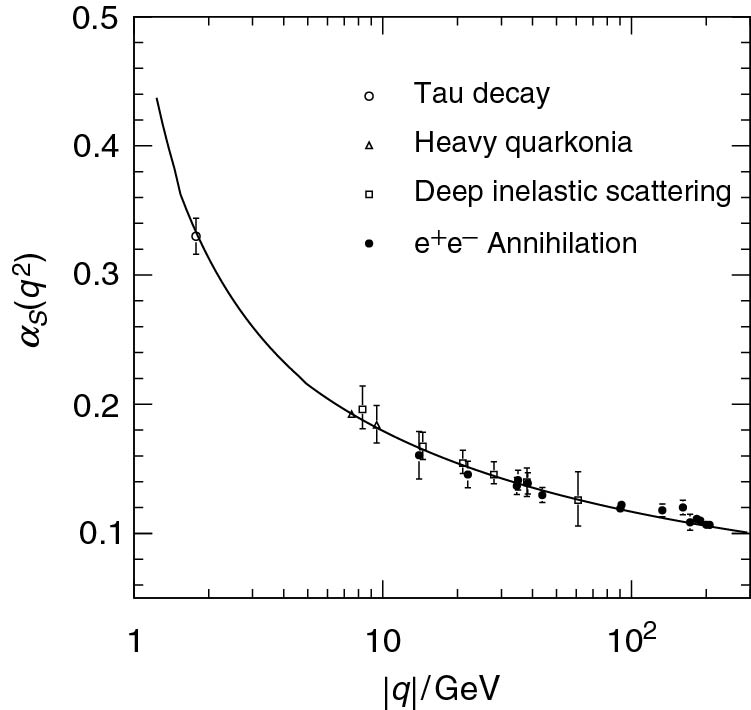
\includegraphics[width=0.3\textwidth]{figs/alphaSrun.png}
  \end{center}
  \item At $q\sim 100~\gev$, QCD enters a perturbative regime
  \item Asymptotic freedom
  \begin{itemize}
    \item Explains why quarks in DIS experiments can be treated as free particles
  \end{itemize}
  \item Running can be measured by looking at jet production at colliders
  \begin{itemize}
    \item e.g. if the $\el\pos\rightarrow q\qbar$ and $\el\pos\rightarrow q\qbar g$ diagrams are included when calculating $R$ (described next section), we get:
    \begin{equation}
      R \rightarrow  \left(1+\frac{\alpha_S(q^2)}{\pi}\right) \times 3\sum_i Q_{q_i}^2
    \end{equation}
    giving a very precise measurement of $\alpha_S(q^2)$
  \end{itemize}
\end{itemize}

\section{Electron-positron annihilation}

\begin{itemize}
  \item First, the inclusive cross-sections for annihilation are (below the $Z$-peak):
  \begin{equation}
    \sigma(\el\pos\rightarrow\mu^-\mu^+) = \frac{4\pi\alpha^2}{s},\quad\sigma(\el\pos\rightarrow q\qbar) = \frac{4\pi\alpha^2}{s}\times 3Q_q^2
  \end{equation}
  \item The inclusive cross-section to hadrons is gotten by summing over all quark flavors satisfying $2m_q < \sqrt{s}$:
  \begin{equation}
    \sigma(\el\pos\rightarrow\text{hadrons}) = \quad\sigma(\el\pos\rightarrow q\qbar) = \frac{4\pi\alpha^2}{s}\times 3\sum_i Q_{q_i}^2
  \end{equation}
  \item Dividing, we get the ratio:
  \begin{equation}
    R(s) = \frac{\sigma(\el\pos\rightarrow \text{hadrons})}{\sigma(\el\pos\rightarrow \mu^-\mu^+)} = 3\sum_i Q_{q_i}^2
  \end{equation}
  For example, $R((2~\gev)^2) = 3\times \left(\frac{3}{9}+\frac{1}{9}+\frac{1}{9}\right) = 2 $
  \item A plot at low values of $\sqrt s$ is:
  \embedimgw{figs/r_thomson.png}{.7}
  The discrete jumps correspond to $\sqrt s = 2m_{q_i}$. The resonances are to $J^P = 1^-$ mesons (needs to be the same as the photon)
\end{itemize}



\embedimgw{figs/ee_xsec.png}{.8}

\section{Electron-proton scattering (elastic)}
\embedimgw{figs/epranges.png}{.5}
\begin{itemize}
  \item The structure probed by the EM interaction depends on the energy of the \el (which determines the $Q^2$ of the interaction)
  \begin{itemize}
    \item At non-relativistic energies, the proton can be described as a point charge
    \item If $1/E_\gamma \sim r_p \sim 1~\fm$, the proton is an extended charge with non-zero $\mu$
    \item At $1/E_\gamma < r_p$, the valence quarks of the proton are probed
    \item And in the limit $1/E_\gamma \ll r_p$, the sea of quarks and gluons is probed
  \end{itemize}
  \item Rutherford scattering
  \begin{itemize}
    \item Non-relativistic limit of \el
    \item If $T_e$ is the kinetic energy of the electron:
    \begin{equation}
      \dd\sigma\Omega = \dfrac{\alpha^2}{16 T_e^2\sin^4(\theta/2)}
    \end{equation}
  \end{itemize}
  \item Mott scattering
  \begin{itemize}
    \item The electron is relativistic, but not so high energy that we need to consider proton recoil, extended charge, etc
    \item $m_e < E_e < m_p$
    \begin{equation}
      \dd\sigma\Omega = \dfrac{\alpha^2}{4E_e^2\sin^4(\theta/2)}\cos^2\frac\theta 2
    \end{equation}
  \end{itemize}
\end{itemize}

\subsection{Form factors}
\begin{itemize}
  \item As $E_\gamma$ increases, we need to account for the extended charge distribution
  \item Write the charge distribution as $Q\rho(\vr')$. Then, the (classical) electric form factor is the Fourier transform of the charge distribution:
  \begin{equation}
    F(\vq^2) = \int d^3r~\rho(\vr) e^{i\vq\cdot\vr}
  \end{equation}
  \item The differential cross-section becomes:
  \begin{equation}
    \left(\dd\sigma\Omega\right)_\text{Mott} \rightarrow \left(\dd\sigma\Omega\right)_\text{Mott} \times \left(F(\vq^2)\right)^2
  \end{equation}
\end{itemize}

\subsection{The Rosenbluth formula}
\begin{itemize}
  \item We now write down the relativistic, leading-order, $\el p$ elastic scattering cross-section:
  \begin{equation}
    \dd\sigma\Omega = \frac{\alpha^2}{4E_1^2\sin^4(\theta/2)}\frac{E_3}{E_1} \left(\frac{G_E^2+\tau G_M^2}{1+\tau}\cos^2\frac\theta 2 + 2\tau G_M^2\sin^2\frac\theta 2\right), \quad \tau = \frac{Q^2}{4m_p^2}
  \end{equation}
  Recall $Q^2 = -q^2$
  \item The form factors $G_E(Q^2)$ and $G_M(Q^2)$ account for the extended charge and magnetic moment distributions inside the proton
  \item As discussed below, the anomalous magnetic moment of the proton is
  \begin{equation}
    \bm\mu = 2.79 \frac{e}{m_p}\Se
  \end{equation}
  so naively, we can guess $G_M(Q^2) = 2.79 G_E(Q^2)$
  \item The $G$s can be measured experimentally. 
  \begin{itemize}
    \item $G_E$ as a function of $Q^2$ can be extracted by measuring the differential cross-section at low $Q^2$ and dividing by the expectation from the Mott formula:
    \begin{equation}
      \dd\sigma\Omega\Big/ \left(\dd\sigma\Omega\right)_\text{Mott} \approx G_E^2 \text{ at low }Q^2
    \end{equation}
    \item Similarly, $G_M$ can be extracted:
    \begin{equation}
      \dd\sigma\Omega\Big/ \left(\dd\sigma\Omega\right)_\text{Mott} \approx \left(1+2\tau\tan^2\frac\theta 2\right) G_M^2 \text{ at high }Q^2
    \end{equation}
    \item Experiment verifies $G_M \approx 2.79 G_E$
  \end{itemize}
  \item By taking the Fourier transform of $G_E(Q^2)$ at low $Q^2$, we can extract the charge distribution:
  \begin{equation}
    \rho(\vr) \approx \rho_0 e^{-r/a}, ~ a = 0.24~\fm
  \end{equation}
  which gives a RMS of $0.8~\fm$
  \item At high $Q^2$, the cross-section goes as:
  \begin{equation}
    \left(\dd\sigma\Omega\right)_\text{elastic} \propto \frac{1}{Q^6} \left(\dd\sigma\Omega\right)_\text{Mott}
  \end{equation}
  so elastic scattering is very suppressed. This is because the proton has finite size and the form factors fall at high $Q^2$. In inelastic scattering, the photon interacts with point particles, which do not have form factors.
\end{itemize}

\section{Electron-proton scattering (inelastic)}
\begin{center}
  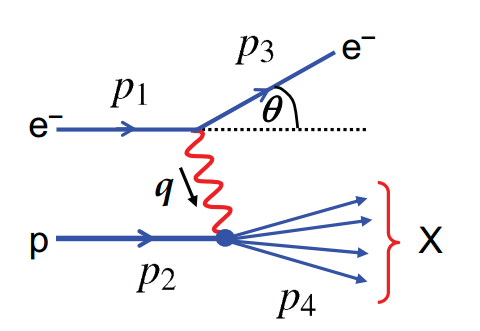
\includegraphics[width=0.3\textwidth]{figs/disfeyn.png}
  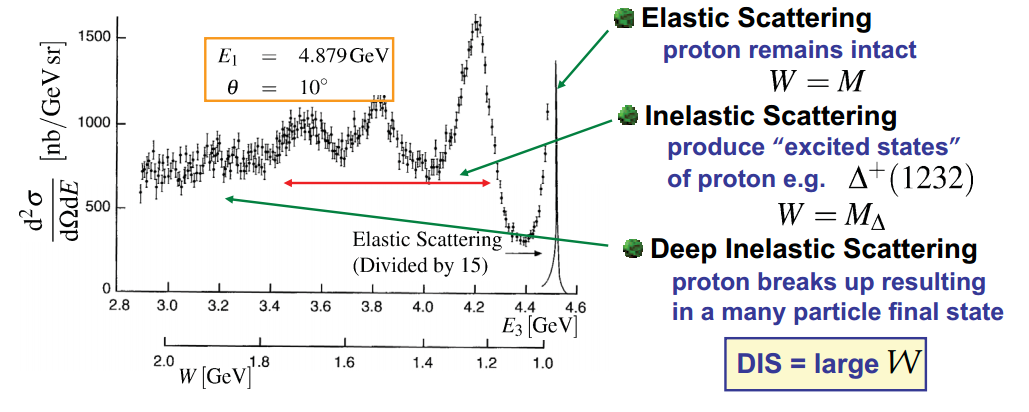
\includegraphics[width=0.6\textwidth]{figs/epxsec.png}
\end{center}
\subsection{Lorentz-invariant kinematic variables}
\begin{itemize}
  \item $Q^2$ is the energy transfer squared
  \begin{equation}
    Q^2 = -q^2
  \end{equation}
  The DIS regime is $Q^2\gtrsim \text{ few}~\gev$
  \item Bjorken $x$ is a measure of the elasticity
  \begin{equation}
    x = \frac{Q^2}{2p_2\cdot q}, ~ x\in [0,1]
  \end{equation}
  Note $x=1$ is the fully elastic scenario (the scattering is probing the proton as a whole)
  \item $W$ is the mass of the hadronic final state
  \begin{equation}
    W^2 = p_4^2 \geq m_p^2
  \end{equation}
  The inequality is because the final state hadronic system must include at least one baryon, and the proton is the lightest baryon
  \item Inelasticity $y$:
  \begin{equation}
    y = \frac{p_2\cdot q}{p_2\cdot p_1}, ~ y\in [0,1]
  \end{equation}
  \item $\nu$
  \begin{equation}
    \nu = \frac{p_2\cdot q}{m_p}
  \end{equation}
  \item The above quantities are obviously not all independent. Knowing two of them specifies the rest. 
\end{itemize}

\subsection{Structure functions}
\begin{itemize}
  \item Can write the DIS cross-section as
  \begin{equation}
    \dd{^2\sigma}{xdQ^2} = \frac{4\pi\alpha^2}{Q^4} \left[(1-y)\frac{F_2(x,Q^2)}{x}+y^2F_1(x,Q^2)\right]
  \end{equation}
  where $F_i$ are the structure functions
  \item The double-differential cross-section can be measured easily at an fixed-target $\el~p$ scattering experiment, since $Q^2,x,y$ are all determined by $E_1, E_3,\theta$ of the electron 
  \begin{itemize}
    \item Can also be done at non-fixed-target experiments; kinematics are just simpler in this case
    \item $F_1(x,Q^2),F_2(x,Q^2)$ are extracted by looking events at fixed $x,Q^2$, and varying $y$. The structure functions can then be extracted from the double-differential cross-section
  \end{itemize}
\end{itemize}

\subsection{Bjorken scaling and the Callan-Gross relation}
\begin{itemize}
  \item Experiments at SLAC did systematic study of $F_i$ as functions of $x,Q^2$
  \begin{itemize}
    \item \el beam (5-20 GeV) fired at liquid hydrogen target
    \item Used movable \el spectrometer to scan $\theta$
  \end{itemize}
  \item Bjorken scaling is the observation:
  \begin{equation}
    F_1(x,Q^2) \sim F_1(x),\quad F_2(x,Q^2)\sim F_2(x)
  \end{equation}
  \begin{itemize}
    \item That is, the structure functions have weak $Q^2$ dependence
    \item Implies that whatever the photon is probing is point-like \thus evidence for quark model
    \item Scaling is violated at very high $Q^2$ (discussed below) \thus quark-gluon interactions
    \begin{itemize}
      \item At high $Q^2$, higher-order QCD interactions become relevant, for example $q\rightarrow qg \rightarrow q$ loops
    \end{itemize}
  \end{itemize}
  \item The same experiments gave the Callan-Gross relation:
  \begin{equation}
    F_2(x) = 2xF_1(x)
  \end{equation}
  \begin{itemize}
    \item Holds true in the DIS regime for $Q^2$
    \item Implies that fundamental interaction is elastic scattering of spin-half particles (i.e. $\el q\rightarrow \el q$)
  \end{itemize}
\end{itemize}

\subsection{Quarks and partons}
\begin{itemize}
  \item The Bjorken $x$ is the fraction of momentum carried by a parton in the ``infinite momentum'' frame.
  \begin{itemize}
    \item In this frame, the proton momentum is $p^\mu = (p,p,0,0)$ (i.e. can ignore the mass)
    \item Let $\xi$ be the fraction of momentum held by the parton. The scattering process is:
    \begin{equation}
      \xi p^\mu \rightarrow \xi p^\mu + q^\mu
    \end{equation}
    \item Since the parton is on-shell before and after:
    \begin{equation}
      (\xi p)^2 =  m_q^2
    \end{equation}
    \begin{equation}
      (\xi p + q)^2 = \xi p^2 + 2\xi p\cdot q + q^2 = m_q^2
    \end{equation}
    \item Equating and solving for $\xi$ gives:
    \begin{equation}
      \xi = \frac{-q^2}{2p\cdot q} = \frac{Q^2}{2p\cdot q} = x
    \end{equation}
  \end{itemize}
  \item The scattering off a spin-half point particle $\el q \rightarrow \el q$ can be written in terms of $y$ and the parton's charge $Q_q$:
  \begin{equation}
    \dd\sigma{Q^2} = \frac{4\pi\alpha^2Q_q^2}{Q^4} \left[(1-y) + \frac{y^2}{2}\right]
  \end{equation}
\end{itemize}

\subsubsection{Parton distribution functions}
\begin{itemize}
  \item Let $q_i^p(x)$ be the probability distribution function of the momentum fraction $x$ held by quarks of flavor $q_i$ in a proton
  \embedimgw{figs/pdfs.png}{.7}
  \item The total $ep$ scattering cross-section is gotten by convoluting the above formula for $d\sigma/dQ^2$ with the PDFs:
  \begin{equation}
    \dd{^2\sigma^{ep}}{xdQ^2} = \frac{4\pi \alpha^2}{Q^4} \left[(1-y)+\frac{y^2}{2}\right] \sum_q Q_i^2 q_i^p(x)
  \end{equation}
  \item We can recover the structure functions from this:
  \begin{equation}
    F_2^{ep}(x,Q^2) = 2xF_1^{ep}(x,Q^2) = x\sum_i Q_i^2 q_i^p(x)
  \end{equation}
  Note that this directly predicts Bjorken scaling and the Callan-Gross relation
  \item Using isospin symmetry, we can define the PDFs for neutrons:
  \begin{gather*}
    u^p(x) = d^n(x) \equiv u(x)\\
    d^p(x) = u^n(x) \equiv d(x)\numberthis
  \end{gather*}
  and similarly for $\ubar(x),\dbar(x)$
  \item Define
  \begin{equation}
    f_q = \int dx~x[q(x)+\qbar(x)]
  \end{equation}
  $f_u,f_d$ can be determined by measuring $F_2^{ep},F_2^{en}$ (neutron scattering is done on deuterium). We find:
  \begin{equation}
    f_u \approx 0.36,~f_d \approx 0.18
  \end{equation}
  in the proton. Therefore, nearly half of the momentum is held in gluons
\end{itemize}

\subsubsection{Sea quarks}
\begin{itemize}
  \item The above discussion only considered $uud$ ($udd$) in protons (neutrons). It can be extended to include sea quarks (considering only $u,d$ now)
  \item First, define:
  \begin{equation}
    q(x) = q_V(x) + q_S(x), \quad \qbar(x) = \qbar_S(x)
  \end{equation}
  \item Since sea quarks are produced in pairs from gluon splitting, we can assume $q_S = \qbar_S$. Since the masses of the $u$ and $d$ are close enough on the DIS energy scale, we can also assume $u_S \approx d_S$
  \item We expect that at very low $x$, sea quarks will dominate the PDFs. In this case:
  \begin{equation}
    \lim_{x\rightarrow 0} \frac{F_2^{en}(x)}{F_2^{ep}(x)} = 1
  \end{equation}
  which was verified at SLAC
\end{itemize}

\subsection{HERA}
  \begin{center}  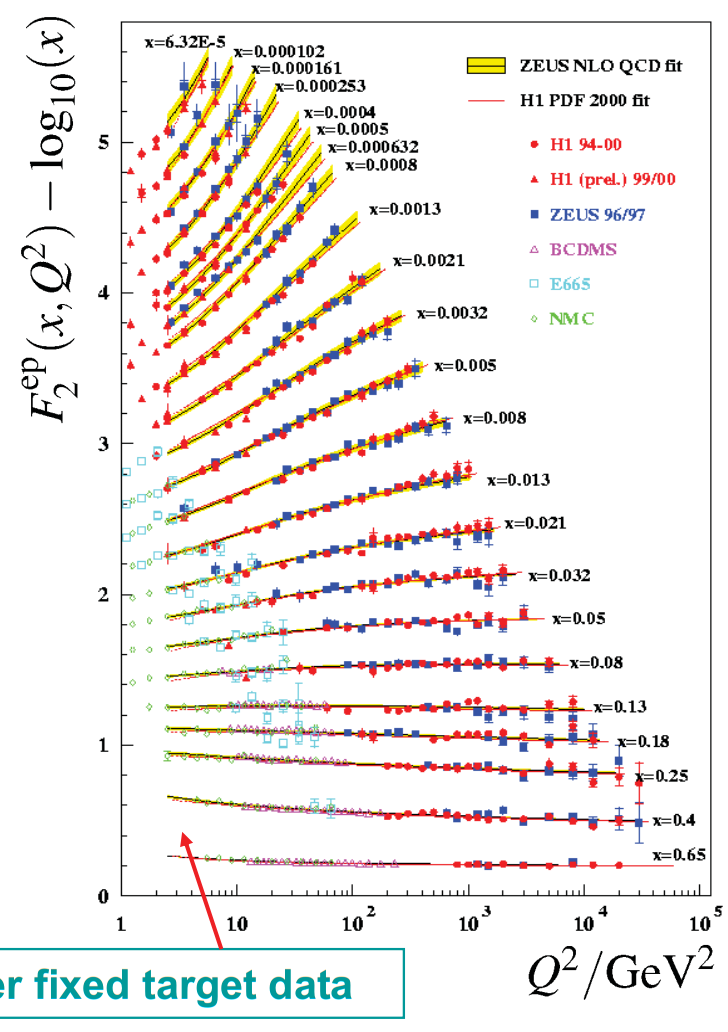
\includegraphics[height=0.7\textwidth,angle=90]{figs/hera.png} \end{center}
\begin{itemize}
  \item $27.5~\gev$ \el/\pos beam colliding with a $820$ or $920$~\gev proton beam
  \item Detector is ``forward'' in the direction of the proton beam
  \item Measured parameters were \el energy and scattering angle \thus sufficient to determine $Q^2,x,y$
  \begin{itemize}
    \item Hadron shower used for trigger only
  \end{itemize}
  \item Huge range of $x,Q^2$ was probed. 
  \item Very powerful evidence of Bjorken scaling 
  \begin{itemize}
    \item There is a violation at low/high $Q^2$, but not consistent across $x$ 
    \item \thus quark radius is $< hc/Q \sim 10^{-18}~\m$
  \end{itemize}
\end{itemize}

\subsubsection{Violation of Bjorken scaling}
\embedimgw{figs/scaleviol.png}{.7}
\begin{itemize}
  \item At high $Q^2$, the photon probes quarks at lower $x$, arising from diagrams like $q\rightarrow qg\rightarrow q$
  \item So at low $x$, the structure function goes up at high $Q^2$; at high $x$, the structure function goes down at high $Q^2$
  \item DGLAP equations describes $Q^2$-dependence
\end{itemize}

\subsubsection{Global PDF fits}
\embedimgw{figs/pdf_global.png}{.5}
\begin{itemize}
  \item Fit is done with information from multiple experiments
  \item Hadron colliders \thus gluon PDF
  \item Can use $\nu N$ experiments to isolate interactions with $u,d$ (depending on $\nu/\nubar$)
\end{itemize}

\section{The weak interaction}
\subsection{Parity violation and the $V-A$ structure}
\subsubsection{Parity violation}
\begin{itemize}
  \item Experimentally observed through the process $^{60}\text{Co}\rightarrow^{60}\text{Ni}^* + \el + \nubar_e$
  \begin{itemize}
    \item Cobalt has permanent nuclear magnetic moment $\mu$, so it can be aligned using an external $B$-field
    \item Wu and collaborators found that the flux of electrons emitted in the same hemisphere as $\vec\mu$ (i.e. $\vec\mu\cdot \vec p_e>0$) is much lower than the flux of electrons emitted in the opposite hemisphere
    \item Under parity, $P:\vec p \mapsto - \vec p$. But since $\vec B,\vec \mu$ are axial vectors, they are invariant under parity. Therefore, the asymmetry represents violation of parity invariance.
  \end{itemize}
  \embedimgw{figs/wu.png}{.4}
\end{itemize}
\subsubsection{$V-A$ structure}
\begin{itemize}
  \item Assuming that the weak interaction is mediated by a spin-1 boson, there are two possible currents: $\psibar \gamma^\mu \psi$ (vector) and $\psibar \gamma^\mu \gamma^5 \psi$ (axial vector)
  \begin{itemize}
    \item Most general form is a linear combination of the two: $j = g_V j_V + g_A j_A$
    \item Can write out all the terms of $j_x\cdot j_y$ (where $x=\nu_e \el$ and $y=du$ for example) and check the effect of $P$
    \item The term that is not invariant under $P$ has a relative strength of 
    \begin{equation}
      \frac{g_Vg_A}{g_V^2+g_A^2}
    \end{equation}
    \item \thus Need $g_V,g_A\neq 0$ to get parity violation
  \end{itemize}
  \item Experimentally, have found the structure to be:
  \begin{equation}
    j^\mu = \frac{g_W}{\sqrt{2}} \ubar(p')\frac{1}{2}\gamma^\mu (1-\gamma^5)u(p)
  \end{equation}
  i.e. $g_V = - g_A$
  \item Chirality consequences of interaction structure:
  \begin{itemize}
    \item Recall for QED that the spinors in particle current $\ubar \gamma^\mu u$ must be both right-handed or both left-handed
    \item The $1-\gamma^5$ in the weak particle current acts as a $P_L$ operator, so both spinors must be left-handed
    \item In the antiparticle current, both must be right-handed.
    \item Note this is also a consequence/cause of parity violation:
    \begin{itemize}
      \item $P:\text{LH} \rightarrow \text{RH}$, one of which interacts weakly while the other does not
    \end{itemize}
  \end{itemize}
\end{itemize}

\subsection{Weak boson kinematics}
\begin{itemize}
  \item Propagator is:
  \begin{equation}
    \frac{-i}{q^2 - m_W^2} \left(g_{\mu\nu} - \frac{q_\mu q_\nu}{m_W^2}\right) \rightarrow \frac{-ig_{\mu\nu}}{q^2-m_W^2}
  \end{equation}
  where the limit is taken assuming $q \ll m_W$, which is generally valid for things like $\beta$-decay, $\nu$ DIS, etc.
  \item Fermi four-point interaction
  \begin{itemize}
      \item Can take the $q\ll m_W$ limit further, so the propagator becomes
      \begin{equation}
        \frac{i g_{\mu\nu}}{m_W^2} 
      \end{equation}
      \item In this case, the interaction no longer depends on the kinematics of the $W$ boson, so it can be treated as a four-point interaction
      \item Historically, it is written in terms of $G_F$, which is:
      \begin{equation}
        \frac{G_F}{\sqrt2} = \frac{g_W^2}{8 m_W^2}
      \end{equation}
      \item Numerically, $G_F = 1.17 \times 10^{-5}~\gev^2$
  \end{itemize}
  \item The dimensionless coupling strength of the weak interaction is:
  \begin{equation}
    \alpha_W \equiv \frac{g_W^2}{4\pi} \approx \frac{1}{30}
  \end{equation}
  which is an order of magnitude larger than $\alpha$
\end{itemize}

\subsection{Pion decay}
\begin{itemize}
  \item Consider the decay of the charged pion (at rest) $\pi^-(\ubar d)\rightarrow \ell \nubar_\ell$
  \item The charged pion is $0^-$, so the $\ell$ and $\nubar_\ell$ must be in the spin-singlet state. 
  \begin{itemize}
    \item If we assume $m_\nu = 0$, a right-handed (chirality) $\nubar$ must also be right-handed (helicity)
    \item Since the decay products are back-to-back, the $\ell$ must also be right-handed (helicity) to be in the spin-singlet state
  \end{itemize}
  \embedimgw{figs/piondecay.png}{.6}
  \item If $m_\ell = 0$, this decay would be forbidden, since only the left-handed (chirality) $\ell$ couples to the weak current. Since this is not the case, there is a small overlap between the right-handed (helicity) and left-handed (chirality) $\ell$ states
  \item The matrix-element of this decay is suppressed due to this small overlap:
  \begin{equation}
    \Mme \sim \frac{m_\ell}{m_\pi + m_\ell}
  \end{equation}
  where $m_\pi = 140~\mev$
  \item Since $m_\mu/m_e \sim 200$, the decay to muons is heavily favored.
  \begin{itemize}
    \item Note that $m_e \ll m_\pi$ is what really drives the suppression, since the electron must be highly relativistic due to the mass difference \thus right-handed (helicity) is almost entirely right-handed (chirality)
  \end{itemize}
  \item The decay rate is proportional to:
  \begin{equation}
    \Gamma (\pi^- \rightarrow \ell \nubar_\ell) \propto \left(m_\ell \left(m_\pi^2 - m_\ell^2\right) \right)^2
  \end{equation}
  So $\Gamma(e)/\Gamma(\mu) \sim 10^{-4}$
  \item Note that this example shows that the weak interaction violates $P$ and $C$, but not $CP$. Consider $\pi^-\rightarrow \nubar_\mu \mu^-$, where the $\nubar_\mu$ is RH (chirality). The muon is as discussed above
  \embedimgw{figs/pioncp.png}{.6}
  % \begin{itemize}
  %   \item If $P$ is applied, the neutrino direction flips but the spin does not (axial vector). Therefore, the neutrino becomes LH (helicity$\approx$chirality). This decay is forbidden
  %   \item If $C$ is applied, the RH (chirality) neutrino becomes a RH (chirality) antineutrino. This decay is forbidden
  %   \item If $CP$ is applied, the RH (chirality) neutrino becomes a LH (chirality) antineutrino. This decay is allowed
  % \end{itemize}
\end{itemize}

\section{Weak interactions of leptons}
\begin{itemize}
  \item Coupling to all three generations is the same (can be verified by measuring at leptonic decays of taus)
\end{itemize}

\subsection{Neutrino scattering}
\begin{itemize}
  \item Can generate beam of $\nu_\mu,\nubar_\mu$ by pointing a proton beam at a target and then using a magnet to select $\pi^-$ or $\pi^+$ 
  \item Mass difference boosts neutrinos along pion direction
  \item Neutrino beam then hits a nucleon target
  \begin{itemize}
    \item $Q^2$ is limited above by $Q^2 \leq 2m_NE_\nu$
    \item $s \approx 2m_NE_\nu$
    \item High-energy neutrino beams typically have $E_\nu = 200-400~\gev$
  \end{itemize}
\end{itemize}
\subsubsection{Nucleon cross-sections}
\begin{itemize}
  \item Angular dependence of cross-sections:
  \begin{gather*}
    \dd{}{\Omega} \sigma_{\nu q},\sigma_{\nubar \qbar} \sim 1\\
    \dd{}{\Omega} \sigma_{\nu \qbar},\sigma_{\nubar q} \sim (1+\cos\theta)^2\numberthis
  \end{gather*}
  \item The $\nu$-$X$ interaction cross-section is always $\sigma\propto s \approx 2 m_X E_\nu$ (where the last approximation is in the limit $m_X\ll E_\nu$ and the target is at rest)
  \item $\sigma_{\nu q} /\sigma_{\nubar q} = 3$ (from integrating the angular dependence)
  \item Note $1-y = \frac{1}{2}(1+\cos\theta)$
\end{itemize}
\subsubsection{Neutrino DIS}
\begin{itemize}
  \item First, define the quark/antiquark PDFs:
  \begin{equation}
    f_q = \int_0^1 dx ~ x[u(x)+d(x)], \quad f_\qbar = \int_0^1 dx ~ x[\ubar(x)+\dbar(x)]
  \end{equation}
  \item Then, the total neutrino-nucleon cross-sections are:
  \begin{gather*}
    \dd{\sigma_{\nu N}}{dy} \propto E_\nu \left[ f_q + (1-y^2) f_\qbar\right]\\
    \dd{\sigma_{\nubar N}}{dy} \propto E_\nu \left[(1-y^2)  f_q + f_\qbar\right]\numberthis
  \end{gather*}
  \item Because $f_q \sim 5 f_\qbar$ in a nucleon, we expect a shape difference in the cross-section
  \item First charged current neutrino DIS was at CDHS
  \begin{itemize}
    \item $\nu_\mu$ beam at scintillator/drift chamber detector. 
    \item Experimental signature is muon track and a large energy deposition in small area (from hadrons)
  \end{itemize}
  \begin{center}
    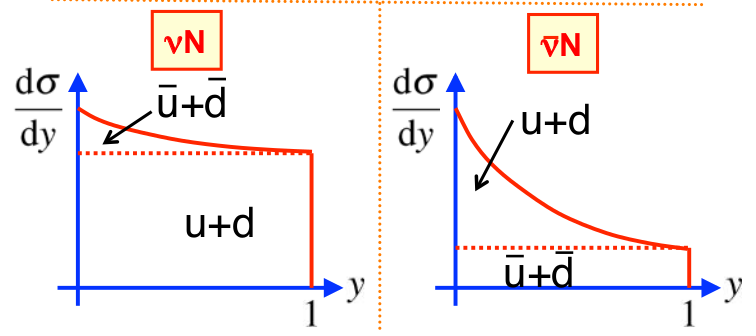
\includegraphics[width=0.5\textwidth,valign=c]{figs/nudis.png}
    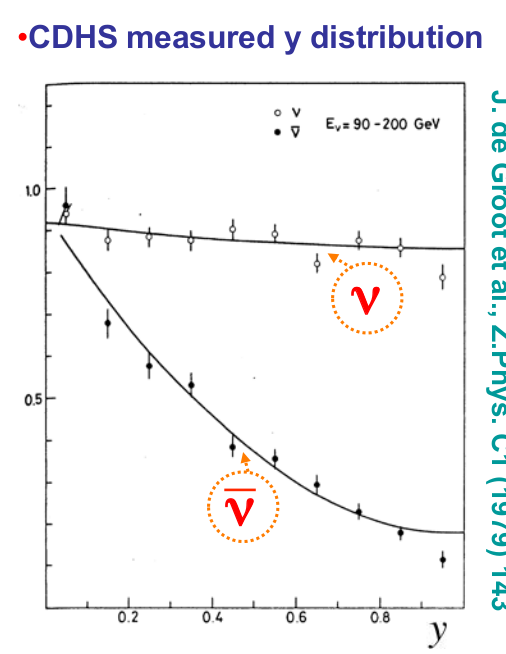
\includegraphics[width=0.3\textwidth,valign=c]{figs/cdhs.png}
  \end{center}
  \item First neutral current interactions were at Gargamelle
  \begin{itemize}
    \item Also a $\nu_\mu$ beam at a bubble chamber detector
    \item Both nucleon DIS and electron scattering were looked for (hadronic shower and free $\el$, respectively)
    \item Reject events with final-state $\mu$ \thus cannot be weak current
  \end{itemize}
\end{itemize}

\subsubsection{Weak contributions to $e$-$p$ scattering}
\begin{itemize}
  \item At high $Q^2$, CC scattering starts to be comparable to (or even dominate) NC (since $\alpha_W > \alpha$)
  \begin{itemize}
    \item Can be differentiated due to different final state: no final state lepton in CC
  \end{itemize}
  \item In general, $\el p$ scattering cross-section is higher than $\pos p$ scattering for two reasons:
  \begin{itemize}
    \item CC: $\el p$ scattering probes high $x$ part of $u_V$ pdf, while $\pos p$ probes $d_V$ pdf (and $u_V(x) > d_V(x)$)
    \begin{itemize}
      \item At low $Q^2$ this difference can be ignored and sea antiquark pdfs become significant
    \end{itemize}
    \item NC: there is $\gamma/Z$ interference at high $Q^2$ which is constructive for $\el p$ and destructive for $\pos p$
  \end{itemize}
\end{itemize}
\embedimgw{figs/weakdis.png}{.4}

\section{Neutrinos and oscillations}
\begin{itemize}
  \item We know that there are different flavors of neutrinos by searching for:
  \embedimgw{figs/mu2e.png}{.3}
  \begin{itemize}
    \item Experiment puts $\text{Br}(\mu\rightarrow\el\gamma)<10^{-11}$
  \end{itemize}
\end{itemize}

\subsection{Solar neutrinos}
\embedimgw{figs/solarnu.png}{.6}
\begin{itemize}
  \item Main source of $\nu_e$
  \item $pp$ reactions:
  \begin{gather*}
    p+p\rightarrow D + \pos +\nu_e \\
    D+p\rightarrow _2^3\text{He} + \gamma \\
    _2^3\text{He}+_2^3\text{He}\rightarrow _2^4\text{He}+p+p \numberthis
  \end{gather*}
  \begin{itemize}
    \item Binding energy of deuteron is only $2.2~\mev$ \thus $E_\nu < 0.5 ~\mev$
    \item Difficult to detect ($\sigma_{\nu N} \propto E_\nu$) so not used in experiments
  \end{itemize}
  \item $\beta$-decay of $^8\text{B}$
  \begin{gather*}
    ^4_2\text{He}+^3_2\text{He}\rightarrow_4^7\text{Be}+\gamma\\
    _4^7\text{Be}+p\rightarrow_5^8\text{B}+\gamma\\
    _5^8\text{B}\rightarrow_4^8\text{Be}^*+\pos+\nu_e\numberthis
  \end{gather*}
  \begin{itemize}
    \item Most used in experiments
    \item $E_\nu$ up to $15~\mev$
  \end{itemize}
  \item Electron capture: $^7\text{Be}+\el \rightarrow ^7\text{Li}+\nu_e$
  \begin{itemize}
    \item Two lines (corresponding to different electron excitations)
    \item Two discrete lines $<1~\mev$
  \end{itemize}
  \item $p+\el+p\rightarrow ^2\text{H}+\nu_e$
  \begin{itemize}
    \item Single line at $1.5~\mev$
  \end{itemize}
\end{itemize}
\subsubsection{Experimental detection}
\begin{itemize}
  \item Homestake
  \begin{itemize}
    \item Large vat of $\text{C}_2\text{Cl}_4$
    \item Flux was measured by counting number of $^{37}\text{Ar}$ atoms
    \item $\nu_e+\text{Cl}\rightarrow \text{Ar}+\el$
    \item Found the solar neutrino problem
    \begin{itemize}
      \item Expected was $1.7$ interactions per day
      \item Found $.5$ interactions per day
    \end{itemize}
  \end{itemize}
  \item Super-Kamiokande
  \begin{itemize}
    \item $50$ kt water Cerenkov detector surrounded by $11$k PMTs
    \item Counts $\nu_e\el\rightarrow\nu_e\el$ events (two leading-order $t$-channel diagrams involving $W$ and $Z$)
    \begin{itemize}
      \item Stability of oxygen nucleus limits CC interaction with oxygen nucleons at low (solar neutrino) energies
    \end{itemize}
    \item Signature is ring of light
    \begin{itemize}
      \item $\el$ is stopped in chamber, so $N_\gamma \propto E_e$
      \item Can discriminate muons (from atmospheric neutrinos) due to sharper ring ($\el$ diffuse more). Muons only arise from NC interactions
    \end{itemize}
    \item Below $E_\nu < 5~\mev$, radioisotope $\beta$-decay backgrounds dominate
    \item Confirms solar neutrino deficit $\sim1/2$ of expected flux
  \end{itemize}
  \item SNO
  \begin{itemize}
    \item Designed to detect electron neutrinos as well as total neutrino flux
    \item Charged current
    \begin{itemize}
      \item $\nu_e +D(pn) \rightarrow \el+p+p$
      \item $\nu_e+\el \rightarrow \nu_e+\el$ (also a NC diagram for this)
      \item Only $\nu_e$ participates because neutrino energies are not high enough to produce $\mu,\tau$
    \end{itemize}
    \item Neutral current
    \begin{itemize}
      \item $\nu_\ell+D(pn)\rightarrow \nu_\ell+p+n$
      \item $\nu_\ell + \el \rightarrow \nu_\ell+\el$
      \item All three flavors participate
    \end{itemize}
    \item Can measure total flux using all processes. Nucleon scattering has higher cross-sections
    \begin{itemize}
      \item Use elastic scattering off electrons to determine fraction of flux that comes from the sun ($\el$ direction is correlated with $\nu$ direction)
    \end{itemize}
    \item Results
    \begin{itemize}
      \item Again, confirms solar neutrino deficit
      \item On the other hand, found that the \emph{total} neutrino flux from the Sun is equal to predicted $\nu_e$ flux \thus first indication of oscillations
    \end{itemize}
  \end{itemize}
\end{itemize}

\subsection{Mass and weak eigenstates}
\begin{itemize}
  \item No reason to expect mass and weak eigenstates of neutrinos to be the same
  \item Mass eigenstates are the physical particle states
  \begin{itemize}
    \item i.e. satisfy $i \partial_t\nu_k = E\nu_k$ for $k=1,2,3$
  \end{itemize}
  \item So a Feynman diagram with an internal $\nu_\ell$ line is really the coherent addition of three diagrams with internal $\nu_k$ lines. If $k=1,2,3$: 
  \embedimgw{figs/internalnulines.png}{.6}
  \item Can define the $\nu_\ell$ states as linear combinations of the particle states:
  \begin{equation}
    |\nu_\ell\ra = \sum_{k=1,2,3} U^*_{\ell k} |\nu_k\ra
  \end{equation}
  \item The $W$ interaction vertex consequently must be written in terms of the mass eigenstates:
  \begin{equation}
    \left(-i U_{\ell k} \frac{g_W}{\sqrt{2}}\right) \bar\ell \gamma^\mu \frac{1}{2} (1-\gamma^5) \nu_k
  \end{equation}
  \begin{itemize}
    \item For interactions involving an outgoing $\nu$ or incoming $\nubar$, $U^*$ is in the vertex factor (i.e. the spinor is in the adjoint rep)
    \item If there is an incoming $\nu$ or outgoing $\nubar$, the spinor is in the fund. rep and $U$ is used
  \end{itemize}
\end{itemize}

\subsubsection{Example: oscillation between two flavors}

\noindent Here is the full derivation for oscillation between two flavors. Suppose there are two flavors $e,\mu$ and two mass eigenstates $1,2$. The free-particle states of the latter propagate as:
\begin{gather}
  |\nu_k(t)\ra = |\nu_k\ra e^{-i p_k\cdot x}
\end{gather}
where $p_k = (E_k,\p_k)$. Let us parametrize $U$ by an angle $\theta$:
\begin{equation}
  \begin{pmatrix} \nu_e \\ \nu_\mu \end{pmatrix} = 
  \begin{pmatrix} \cos \theta & \sin\theta \\ -\sin\theta & \cos\theta \end{pmatrix}
  \begin{pmatrix} \nu_1 \\ \nu_2 \end{pmatrix} 
\end{equation}
Suppose $\nu_e$  is produced at $t=0$:
\begin{equation}
  |\nu(0)\ra = |\nu_e \ra = \cos\theta|\nu_1\ra + \sin\theta|\nu_2\ra
\end{equation}
The evolution is then given by the free particle equation above:
\begin{equation}
  |\nu(x)\ra = \cos\theta |\nu_1\ra e^{-ip_1\cdot x} + \sin\theta |\nu_2\ra e^{-ip_2\cdot x}
\end{equation}
Now suppose the neutrino interacts weakly at a distance $L$ and time $T$. It will be projected into a weak eigenstate. At this point, the wavefunction is:
\begin{equation}
  |\nu(T,L)\ra = \cos\theta |\nu_1\ra e^{-i\phi_1} + \sin\theta |\nu_2\ra e^{-i\phi_2}, \quad \phi_k = E_k T - p_k L
\end{equation}
If we invert $U$ and plug into the above equation:
\begin{align*}
  |\nu(T,L)\ra &= \cos\theta e^{-i\phi_1}\left[\cos\theta |\nu_e\ra - \sin\theta|\nu_\mu\ra\right] + \sin\theta e^{-i\phi_2}\left[\sin\theta |\nu_e\ra + \cos\theta|\nu_\mu\ra\right]\\
  &= e^{-i\phi_1} \left( \left[\cos^2\theta+ e^{i\Delta\phi_{12}}\sin^2\theta\right]|\nu_e\ra + \left[1-e^{i\Delta\phi_{12}}\right]\sin\theta\cos\theta|\nu_\mu\ra \right) \numberthis
\end{align*}
where
\begin{equation}
  \Delta\phi_{12} = \phi_1 - \phi_2
\end{equation}
If $\Delta\phi_{12} \neq 0$, the $\nu_\mu$ projection is non-zero. Squaring the factor multiplying $|\nu_\mu\ra$, we get:
\begin{equation}
  P(\nu_e\rightarrow \nu_\mu) = \sin^2(2\theta) \sin^2 \left(\frac{\Delta\phi_{12}}{2}\right)
\end{equation}
There are different assumptions one could make in calculating $\Delta\phi_{12}$ (in principle, one should evolve wavepackets instead of free particles). Here we assume $p_1 = p_2$, but one could also assume $E_1 = E_2$ or $\beta_1 = \beta_2$ and get the same answer.
\begin{align*}
  \Delta\phi_{12} &= (E_1-E_2)T - (p-p)L = \left[\sqrt{p^2+m_1^2} - \sqrt{p^2+m_2^2}\right]T\\
    &\approx \left[p \left(1+ \frac{m_1^2}{2p^2}\right) - p \left(1+ \frac{m_1^2}{2p^2}\right)\right]T\\
    &= \left(m_1^2-m_2^2\right) \frac{L}{2p} \equiv \Delta m^2_{12} \frac{L}{2E_\nu} \numberthis
\end{align*}
In the last line, we assume $\beta \approx 1$ and $p\approx E_\nu$. 

\subsubsection{Oscillation between three flavors}
\begin{itemize}
  \item The calculation is similar to above, but more complicated
  \begin{itemize}
    \item Have to deal with the fact that things like $e\rightarrow\mu\rightarrow \tau$ can happen, affecting the oscillation probabilities
  \end{itemize}
  \item The matrix is known as the PMNS matrix
  \item The phase differences are defined as:
  \begin{equation}
    \Delta_{ij} = (m_i^2-m_j^2) \frac{L}{4E_\nu} \equiv \Delta m_{ij}^2 \frac{L}{4E_\nu}
  \end{equation}
  Note tat they are not all independent. We can write $\Delta_{31} = \Delta_{32} + \Delta_{21}$
  \item The survival probability is:
  \begin{equation}
    P(\nu_e\rightarrow\nu_e) = 1 - 4|U_{e1}|^2|U_{e2}|^2 \sin^2\Delta_{21} - 4|U_{e1}|^2|U_{e3}|^2 \sin^2\Delta_{31} - 4|U_{e2}|^2|U_{e3}|^2 \sin^2\Delta_{32}
  \end{equation}
\end{itemize}

\subsubsection{Neutrino masses}
\begin{itemize}
  \item Neutrino oscillation experiments are only sensitive to \emph{difference} in squared masses, not the masses themselves
  \item Looking at end-point of electron $Q$ distribution in tritium $\beta$-decay shows that the lightest eigenstate must be $\lesssim 2~\ev$
  \item Large-scale structure and measurement of C$\nu$B limit $\sum_k m_{k} \lesssim 1~\ev$
  \item Best measurements of mass differences are:
  \begin{gather*}
    \Delta m_{21}^2 \sim 10^-4~\ev^2\\
    \Delta m_{32}^2 \sim 10^-3~\ev^2\numberthis
  \end{gather*}
  \begin{itemize}
    \item The sign of $\Delta m_{32}^2$ is unknown. $m_3>m_2$ is the normal hierarchy; the inverse is the inverted hierarchy.
    \embedimgw{figs/nuhierarchy.png}{.6}
    \item $\Delta m_{31}^2$ has not been measured independently.
  \end{itemize}
\end{itemize}

\subsubsection{$CP$ violation}
\begin{itemize}
  \item Recall that QED and QCD conserve $C$ and $P$ separately, so they cannot lead to $CP$ violation. Weak interactions could be a source of $CP$ violation.
  \item Two ways of determining if $CP$ violation occurs in the PMNS matrix:
  \begin{itemize}
    \item Measure $P(\nu_e\rightarrow\nu_\mu)$ and the $CP$-transformed quantity $P(\nubar_e\rightarrow\nubar_\mu)$ (note $C$ is not enough since you would go from LH $\nu$s to RH $\nubar$s). Measure the difference in the probabilities; it should be $0$ if $CP$ is not violated
    \item Assuming $CPT$ invariance, $CP$ violation implies $T$ violation. Therefore, one could measure $P(\nu_\mu\rightarrow \nu_e)$ and check it is equal to $P(\nu_e\rightarrow\nu_\mu)$
  \end{itemize}
  \item In order for this to occur, elements of the PMNS matrix must have imaginary components. There is in fact only one independent complex phase in the matrix (the others can be absorbed into particle definitions):
  \begin{equation}
    \begin{pmatrix} 
      U_{e1} & U_{e2} & U_{e3} \\
      U_{\mu1} & U_{\mu2} & U_{\mu3} \\
      U_{\mu1} & U_{\mu2} & U_{\tau3} 
    \end{pmatrix} = 
    \begin{pmatrix} 
      c_{12}c_{13} & s_{12}s_{13} & s_{13}e^{-i\delta} \\
      -s_{12}c_{23}-c_{12}s_{23}s_{13}e^{i\delta} & c_{12}c_{23}-s_{12}s_{23}s_{13}e^{i\delta} & s_{23}c_{13}\\
      -s_{12}s_{23}-c_{12}c_{23}s_{13}e^{i\delta} & c_{12}s_{23}-s_{12}c_{23}s_{13}e^{i\delta} & c_{23}c_{13}
    \end{pmatrix}   
  \end{equation}
  \item Current experiments are not sensitive to $CP$ violation in the neutrino sector
\end{itemize}

\section{Oscillation experiments}
\begin{itemize}
  \item Both neutrinos and antineutrinos have $t$-channel CC and NC interactions with electrons and nucleons
  \begin{itemize}
    \item Antineutrinos also have a $s$-channel CC interaction $\nubar_e \el \rightarrow \nubar_e \el$
  \end{itemize}
  \item Muon neutrinos interact with electrons through CC only if $E_{\nu_\mu}>11~\gev$ (need to be able to create the muon). Threshold for taus is $3~\tev$
\end{itemize}

\subsection{Reactor experiments}
\begin{itemize}
  \item Use $\nubar_e$ flux from $\beta^-$ decays of $^{235}\text{U},~^{238}\text{U},~^{239}\text{Pu},~^{241}\text{Pu}$
  \begin{itemize}
    \item Flux is precisely known from power output of reactor
    \item Energies are $\sim\mev$, so nucleon CC interaction is inverse $\beta$ decay (as opposed to DIS)
  \end{itemize}
  \item Because energies are too low to produce $\mu,\tau$ in either nucleon or electron interactions, oscillation is observed through deficit of $\nubar_e$
  \item Two oscillation wavelengths
  \begin{itemize}
    \item Long-wavelength: sensitive to $\Delta m_{21}^2,\theta_{12}$. This is what solar neutrino experiments are sensitive to. $\ord{100}$ km
    \item Short-wavelength: sensitive to $\Delta m_{32}^2,\theta_{13}$. $\ord1$ km
  \end{itemize}
\end{itemize}
\embedimgw{figs/nue_probability.png}{.5}

\subsubsection{Short baseline}
\begin{itemize}
  \item Sensitive to only short-wavelength oscillations
  \begin{equation}
    P(\nubar_e\rightarrow \nubar_e) \approx 1- \sin^2(2\theta_{13}) \sin^2 \left(\frac{\Delta m_{32}^2 L}{4E_\nubar}\right)
  \end{equation}
  \item Daya Bay
  \begin{itemize}
    \item Detectors positioned at various distances from reactor cores ($470, 580, 1650$ m away)
    \item Detector is liquid scintillator loaded with Gd, surrounded by PMTs
    \item Inverse $\beta$-decay has highest cross-section ($\nubar_e+p\rightarrow \pos+n$)
    \item Signal signature
    \begin{itemize}
      \item $\pos$ annihilates with an $\el$ and releases two prompt photons
      \item Low energy $n$ drifts for a while until capture by a Gd nucleus, which then de-excites and releases a photon (timescale of $100~\mus$)
    \end{itemize}
    \item Assuming known value of $\Delta m_{32}^2$, Daya Bay measures:
    \begin{equation}
      \sin^2(2\theta_{13}) = 0.10 \pm 0.01
    \end{equation}
  \end{itemize}
  \item KamLAND
  \begin{itemize}
    \item Scintillator-PMT detector at 130-240 km away from reactor core
    \item Again, I$\beta$D is dominant process
    \item Signal signature
    \begin{itemize}
      \item Two prompt photons from $\pos$ annihilation
      \item Delayed $2.2~\mev$ photon from $n+p\rightarrow D+\gamma$
    \end{itemize}
    \item Measured $\Delta m_{21}^2\sim 8\times 10^{-5}~\ev^2$ and $\sin^2(2\theta_{12})=0.87$
  \end{itemize}
\end{itemize}

\subsubsection{Long baseline}
\begin{itemize}
  \item Relies on accelerator-based neutrino beams
  \item Use one near and one far detector. Systematic uncertainties will be the same, so can assume they cancel in the ratio when measuring survival probabilities
  \item MINOS
  \begin{itemize}
    \item High intensity $\nu_\mu$ beam from Fermilab
    \begin{itemize}
      \item $E_\nu \sim 1\text{-}5~\gev$
      \item $L=735$ km
    \end{itemize}
    \item Dominant interaction is $\nu_\mu N\rightarrow\mu^-+$hadrons
    \item Detector is planes of iron with plastic scintillator inbetween
    \begin{itemize}
      \item Magnetic field to curve charge particles
      \item Muon is identified and $p_\mu$ is measured by looking for a long curved track (hadrons will be stopped quickly)
      \item $E_\text{had}$ is measured by amount of scintillation light near beginning of muon track (interaction vertex)
    \end{itemize}
    \item At these energies, the oscillation associated with $\Delta_{21}$ is much longer than $L$ so can be ignored. Since $\theta_{13}$ is tiny, only $\mu,\tau$ need to be considered
    \item $\nu_\tau$ energies are too low to produce a $\tau$, so oscillation is measured by looking for a deficit of $\nu_\mu$ interactions
    \item Measures $|\Delta m_{32}^2| = 2.3 \times 10^{-3}~\ev^2$ and $\sin^2(2\theta_{23})\gtrsim 0.9$
  \end{itemize}
\end{itemize}

\subsection{Global picture}
\begin{itemize}
  \item Mass differences measured to within $5\%$:
  \begin{itemize}
    \item $\Delta m_{21}^2 = 7.6 \times 10^{-5}~\ev^2$
    \item $\Delta m_{32}^2 = 2.3 \times 10^{-3}~\ev^2$
  \end{itemize}
  \item Three of the four PMNS parameters are measured (or are constrained):
  \begin{itemize}
    \item $\sin^2(2\theta_{12}) = 0.87$
    \item $\sin^2(2\theta_{23}) > 0.92$
    \item $\sin^2(2\theta_{13}) > 0.10$
  \end{itemize}
  \item The CP violating phase $\delta$ is not constrained at all
  \item Best measurement is:
  \begin{equation}
    \begin{pmatrix} \nu_e \\ \nu_\mu \\ \nu_\tau \end{pmatrix} = \begin{pmatrix} 0.82 & 0.54 & 0.15 \\ 0.35 & 0.70 & 0.62 \\ 0.44 & 0.45 & 0.77 \end{pmatrix}\begin{pmatrix} \nu_1 \\ \nu_2 \\ \nu_3 \end{pmatrix}
  \end{equation}
\end{itemize}

\section{Weak interactions of quarks}
\subsection{$CP$ violation and baryogenesis}
\begin{itemize}
  \item If there was no \CP violation in the early universe, we would expect $n_B = n_{\bar{B}}$
  \begin{itemize}
    \item Early universe was in thermal equilibrium with $\gamma+\gamma \leftrightarrow B+\bar{B}$ occurring at equal rates
    \item As universe cooled and $k_BT< 2 m_B$, the forward process stopped, freezing $n_B,n_{\bar{B}}$
  \end{itemize}
  \item Experimentally, we measure:
  \begin{equation}
    \xi = \frac{n_B- n_{\bar{B}}}{n_\gamma} \approx \frac{n_B}{n_\gamma} \sim 10^{-9}
  \end{equation}
  \item Can be explained by very small asymmetry in early universe
  \begin{itemize}
    \item For example, if $n_{\bar{B}} = 10^9$ and $n_B = 10^9+1$ in the early universe
    \item If the baryons and antibaryons annihilated, today $n_{\bar{B}} = 0, n_B = 1, n_\gamma \sim 10^9$, giving the observed value of $\xi$
  \end{itemize}
  \item Three conditions need to be met to make this mechanism work:
  \begin{itemize}
    \item $A = n_B - n_{\bar{B}}$ is not constant
    \item $C$ and \CP must be violated. If \CP is conserved and there is a process that increases $A$, there would be a \CP conjugate process decreasing it
    \item Lack of thermal equilibrium. If the universe remained at thermal equilibrium, then any process that increases $A$ would be canceled by the reverse process
  \end{itemize}
\end{itemize}

\subsection{Cabbibo mixing and the weak interaction}
\begin{itemize}
  \item Let us start by assuming that the coupling of the weak interaction to \emph{quark weak eigenstates} is universal. It turns out this is in agreement with observation
  \item Consider for now that there are only two generators of quarks
  \item As is the case for neutrinos, the down-type quark weak eigenstates are not the same as the mass eigenstates. Let $q'$ be the weak eigenstates. Then:
  \begin{equation}
    \begin{pmatrix} d' \\ s' \end{pmatrix}
     = \begin{pmatrix} \cos\theta_C & \sin\theta_C \\ -\sin\theta_C & \cos\theta_C \end{pmatrix}
    \begin{pmatrix} d \\ s \end{pmatrix}
  \end{equation}
  where $\theta_C\approx 13^o$ is the Cabbibo angle ($\cos\theta_C \approx 0.97$)
  \item The weak interaction vertices are modified accordingly. For example, the vertex factor for $W^+\rightarrow \dbar c$ is $-\frac{g_W}{\sqrt2}\sin\theta_C$ (note $\dbar$ refers to the \emph{mass} eigenstate and $-\sin\theta_C$ is the overlap between $d$ and $s'$)
  \item The exact value of $\cos\theta_C$ can be extracted from the rate of nuclear $\beta$ decay, for example
  \item Kaon decay and GIM mechanism
  \embedimgw{figs/kLdecay.png}{.6}
  \begin{itemize}
    \item Consider the decay $K_L \rightarrow \mu^+\mu^-$. It can proceed through the box diagram on the left in the figure above. The matrix element is proportional to:
    \begin{equation}
      \Mme \propto g_W^4\cos\theta_C\sin\theta_C
    \end{equation}
    \item However, the observed BR is much \emph{smaller} than would be expected from this one diagram. When this was observed, the $c$ quark had not been discovered.
    \item However, if we include the $c$ quark and use the Cabbibo mixing matrix, then we get the diagram on the right. The matrix element is:
    \begin{equation}
      \Mme \propto -g_W^4\cos\theta_C\sin\theta_C
    \end{equation}
    Note the minus sign is from the $d,s'$ element of the matrix
    \item Adding these matrix elements leads to a cancellation. The cancellation is not exact because the matrix element includes kinematic factors (which are slightly different for a virtual $u$ and $c$)
  \end{itemize}
\end{itemize}

  \subsection{The CKM matrix}
  \begin{itemize}
    \item We can extend the above argument to three generations using the CKM matrix:
    \begin{equation}
      \begin{pmatrix} d' \\ s' \\ b' \end{pmatrix} = 
      \begin{pmatrix} V_{ud} & V_{us} & V_{ub}\\
      V_{cd} & V_{cs} & V_{cb}\\
      V_{td} & V_{ts} & V_{tb} \end{pmatrix}
      \begin{pmatrix} d \\ s \\ b \end{pmatrix}
    \end{equation}
    \item Vertex factors are modified accordingly. If the up-type quark is leaving the interaction, use $V$; otherwise use $V^*$
    \item Like the PMNS matrix, the CKM matrix is parametrized by three angles ($\phi_{12},\phi_{23},\phi_{13}$) and a phase shift ($\delta'$)
    \item The magnitude of each element of $V$ can be measured independently:
    \begin{itemize}
      \item $V_{ud}$: superallowed $0^+\rightarrow 0^+$ nuclear $\beta$ decays
      \item $V_{us}$: decay rate of $K_L^0(d\sbar) \rightarrow \pi^-(d\ubar) + \pos\nu_e$
      \item $V_{ub}$: decay rate of $B^0(d\bbar)\rightarrow  \pi^-(d\ubar) + \pos\nu_e$
      \item $V_{cd}$: cross-section of $\nu_\mu d \rightarrow \mu^- c$, where the $c$ is identified by its decay to $s \mu^+ \nu_\mu$.
      \item $V_{cs}$: decay rate of $D^+_s(c\sbar)\rightarrow \mu^+\nu_\mu$
      \item $V_{cb}$: decay rate of B mesons to final states with charm
      \item $V_{td}$ and $V_{ts}$: oscillation rate of $B^0\leftrightarrow \bar B^0$ 
      \item $V_{tb}$: decay rate of $t\rightarrow bW$ (large uncertainties)
    \end{itemize}
    \item The observed magnitudes are:
    \begin{equation}
      |V| = \begin{pmatrix} 0.974 & 0.225 & 0.004\\
      0.225 & 0.973 & 0.041\\
      0.009 & 0.040 & 0.999 \end{pmatrix}
    \end{equation}
  \end{itemize}

  \subsection{Neutral kaon system}
  \begin{itemize}
    \item Neutral kaons ($d\sbar$ and $s\dbar$) can be produced strongly:
    \begin{align*}
      \pi^-(d\ubar) + p(uud) &\rightarrow \Lambda(uds)+K^0(d\sbar)\\
      p(uud)+\bar p(\ubar\ubar\dbar) &\rightarrow K^+(u\sbar) + \bar K^0 (s\dbar) + \pi^-(d\ubar)\numberthis
    \end{align*}
    Thus, $K^0,\bar K^0$ are strong (flavor) eigenstates
    \item Neutral kaons are the lightest charged bound states, so they must decay weakly.
    \begin{itemize}
      \item For mass reasons, the decay must be leptonically or to pions
      \item Neutral kaons can also mix with each other:
      \embedimgw{figs/kaonmixing.png}{.7}
    \end{itemize}
    \item Therefore, the physical states are not $K^0, \bar K^0$: if a $K^0$ is produced, it will not stay a $K^0$. Physical states only evolve through phase rotations
    \item The real physical states are linear combinations of $K^0,\bar K^0$. Call them $K_S,K_L$. It turns out their masses are quite close ($\sim 498~\mev$), but their lifetimes are quite different:
    \begin{equation}
      \tau_{K_S} \sim 10^{-9}~\s ~< ~\tau_{K_L} \sim 10^{-7}~\s
    \end{equation}
  \end{itemize}

  \subsubsection{Kaon \CP eigenstates}
  \begin{itemize}
    \item On the road to constructing $K_S,K_L$, let us first figure out the \CP eigenstates of the system
    \item The action of \CP is:
    \begin{equation}
      \CP \begin{pmatrix} K^0 \\ \bar K^0 \end{pmatrix} = \begin{pmatrix} \bar K^0 \\ K^0 \end{pmatrix}
    \end{equation}
    implying that the \CP eigenstates are:
    \begin{equation}
      K_1 = \frac{K^0 + \bar K^0}{\sqrt2},\quad K_2 = \frac{K^0 - \bar K^0}{\sqrt2}
    \end{equation}
    \item The \CP of $K_1$ ($K_2$) is $+1$ ($-1$)
    \item If \CP were conserved, $K_S,K_L$ would be the same as $K_1,K_2$. However, due to a weak \CP violation, this equality is close but not exact
  \end{itemize}

  \subsubsection{Kaon decays to pions}
  \begin{itemize}
    \item It is observed that $K_S$ decays to two neutral pions much faster than it decays to three neutral pions; the converse is true for $K_S$
    \item $K_{S,L}\rightarrow \pi^0\pi^0$ or $\pi^+\pi^-$
    \begin{itemize}
      \item Since neutral kaons and pions are $J^P = 0^-$, the angular momentum of the final state must be $l=0$
      \item \thus \CP of the final state is +1 (true for either final state)
    \end{itemize}
    \item $K_{S,L} \rightarrow \pi^0\pi^0\pi^0$ or $\pi^+\pi^-\pi^0$
    \begin{itemize}
      \item Similar arguments can be made to show the final state is $\CP = -1$
    \end{itemize}
    \item If \CP were conserved (which it almost is):
    \begin{itemize}
      \item The only way to get to the two-pion (\CP-even) final state is to start with $K_1$
      \item The only way to get to the three-pion (\CP-odd) final state is to start with $K_2$
    \end{itemize}
    \item The decay to two pions is obviously favored for mass reasons, so $K_1$ decays much faster than $K_2$
    \begin{equation}
      m_K - 2m_\pi = 220~\mev ~ > ~ m_K - 3m_\pi = 80~\mev
    \end{equation}
    \item Because \CP is slightly violated, the decays $K_L\rightarrow \pi\pi$ and $K_S \rightarrow \pi\pi\pi$ are not forbidden, just very suppressed
  \end{itemize}

  \subsubsection{\CP violation in kaons}
  \begin{itemize}
    \item Can be detected in the following way (\`a la Cronin and Fitch):
    \begin{itemize}
      \item Start with a beam of pure $K^0$ (or $\bar K^0$). Can be achieved in $p\bar p$ collisions as described above
      \item Allow the beam to travel for a distance $L\gg c\tau_S$, so that all the $K_S$ have decayed
      \item Look for two-pion decays in the remaining beam of $K_L$
      \item Found to be $\sim 0.3\%$ (inclusive)
    \end{itemize}
    \item Two ways of introducing \CP violation: in the mixing of $K^0\leftrightarrow \bar K^0$ or in the decay of the \CP eigenstate itself
    \item \CP violation in kaon mixing
    \begin{itemize}
      \item This turns out to be the dominant effect and is due to \CP violation in the CKM matrix
      \item The mass eigenstates are:
      \begin{equation}
        K_S = \frac{K_1 + \epsilon K_2}{\sqrt{1+|\epsilon|^2}},\quad K_L = \frac{\epsilon K_1 +  K_2}{\sqrt{1+|\epsilon|^2}}
      \end{equation}
      for a small complex parameter $\epsilon$
    \end{itemize}
    \item \CP violation in kaon decay
    \begin{itemize}
      \item Also due to \CP-violating phase in CKM matrix
      \item Parametrized by $\epsilon'$. NA48 and KTeV measure:
      \begin{equation}
        \mathfrak{Re} \frac{\epsilon'}{\epsilon} \sim 10^{-3}
      \end{equation}
    \end{itemize}
  \end{itemize}

\begin{appendices}
\section{Bibliography}
~
\bibspace Klute M., \emph{Lecture notes from 8.811}. Fall 2015
\bibspace PDG Particle Review, \emph{Plots of cross sections and related quantities}. 2015
\bibspace PDG Particle Review, \emph{CKM quark-mixing matrix}. 2015
\bibspace Tapper A., \emph{High $Q^2$ neutral current cross sections in $\el p$ DIS}. \url{http://www.hep.ph.imperial.ac.uk/~tapper/talks/dis04.pdf}
\bibspace Thomson M., \emph{Modern Particle Physics}
\bibspace Thomson M., \emph{Online lecture notes} (\url{http://www.hep.phy.cam.ac.uk/~thomson/partIIIparticles/welcome.html})
\bibspace Universitat Heidelberg, \emph{Solar neutrino problem}. \url{http://www.kip.uni-heidelberg.de/tt_detektoren/neutrinos.php?lang=en}

\end{appendices}

\end{document}
